import os

LATEX_PREAMBLE = r"""\documentclass[aspectratio=169,10pt]{beamer}

% ==============================================================================
% THEME & ENGINE SETUP (Minimalist Academic Lecture Style)
% ==============================================================================
\usetheme{Boadilla}
\usecolortheme{dove}

\usepackage[utf8]{inputenc}
\usepackage[T1]{fontenc}
\usepackage{lmodern}
\usepackage{helvet}
\renewcommand{\familydefault}{\sfdefault}
\usepackage{booktabs}
\usepackage{tabularx}
\usepackage{array}
\usepackage{colortbl}
\usepackage{amsmath,amssymb}
\usepackage{tikz}
\usepackage{pgfplots}
\pgfplotsset{compat=1.18}
\usetikzlibrary{arrows.meta,positioning,calc,fit,shapes.geometric}

% ==============================================================================
% MINIMALIST ACADEMIC COLOR PALETTE (Black/White/Gray with Blue & Red Accents)
% ==============================================================================
\definecolor{inkBlack}{RGB}{17, 24, 39}       % Charcoal Black (Primary Text)
\definecolor{inkDark}{RGB}{55, 65, 81}        % Slate Gray (Headings & Labels)
\definecolor{inkMuted}{RGB}{107, 114, 128}    % Neutral Gray (Captions & Footers)
\definecolor{inkLight}{RGB}{248, 249, 250}    % Clean Light Gray Fill (Panels & Cards)
\definecolor{inkRule}{RGB}{218, 222, 229}     % Subtle Divider & Border Line
\definecolor{focusBlue}{RGB}{29, 78, 216}     % Cobalt Blue (Primary Path & Success Accent)
\definecolor{focusRed}{RGB}{185, 28, 28}      % Crimson Red (Bottleneck & Alert Accent)

% ==============================================================================
% BEAMER LAYOUT & TYPOGRAPHY SETTINGS
% ==============================================================================
\setbeamercolor{background canvas}{bg=white}
\setbeamercolor{normal text}{fg=inkBlack}
\setbeamercolor{structure}{fg=focusBlue}
\setbeamercolor{frametitle}{fg=inkBlack}
\setbeamercolor{item}{fg=focusBlue}
\setbeamertemplate{navigation symbols}{}
\setbeamertemplate{itemize items}[circle]

% Clean Frametitle Banner
\setbeamertemplate{frametitle}{
    \vspace{0.25cm}
    \begin{beamercolorbox}[wd=\paperwidth,leftskip=0.8cm,rightskip=0.8cm]{frametitle}
        {\fontsize{5.5pt}{6.5pt}\selectfont\color{focusBlue}\textbf{\MakeUppercase{\insertsection}}\strut\par}\vspace{1pt}
        {\fontsize{11.5pt}{13.5pt}\selectfont\bfseries\color{inkBlack}\insertframetitle\strut\par}
        \ifx\insertframesubtitle\@empty\else
            \vspace{1pt}{\fontsize{7.5pt}{9.5pt}\selectfont\color{inkMuted}\insertframesubtitle\strut\par}
        \fi
    \end{beamercolorbox}
    \vspace{-0.15cm}
}

% Minimal Footline
\setbeamertemplate{footline}{
    \leavevmode
    \hbox{
        \begin{beamercolorbox}[wd=0.55\paperwidth,ht=2.5ex,dp=1.1ex,leftskip=0.8cm]{normal text}
            \fontsize{5.5pt}{6.5pt}\selectfont\color{inkMuted}\textbf{TuneTrace: Adaptive Music Recommendation System} \textbar\ Review 1 Evaluation
        \end{beamercolorbox}
        \begin{beamercolorbox}[wd=0.45\paperwidth,ht=2.5ex,dp=1.1ex,rightskip=0.8cm]{normal text}
            \hfill\fontsize{5.5pt}{6.5pt}\selectfont\color{inkMuted}Agrannya Singh (23BCE0965) \quad\textbar\quad Slide \insertframenumber{} of \inserttotalframenumber
        \end{beamercolorbox}
    }
    \vspace{0.15cm}
}

\begin{document}

% ==============================================================================
% SLIDE 1: TITLE SLIDE
% ==============================================================================
\begin{frame}[plain]
    \begin{tikzpicture}[remember picture,overlay]
        \draw[inkBlack, line width=1.2pt] ($(current page.north west)+(0.8cm, -0.8cm)$) -- ($(current page.north east)+(-0.8cm, -0.8cm)$);
        \draw[inkRule, line width=0.5pt] ($(current page.south west)+(0.8cm, 1.4cm)$) -- ($(current page.south east)+(-0.8cm, 1.4cm)$);
    \end{tikzpicture}

    \vspace{0.6cm}
    \begin{beamercolorbox}[wd=\textwidth,left]{title}
        {\fontsize{6.5pt}{7.5pt}\selectfont\color{focusBlue}\textbf{\MakeUppercase{Project Review 1 Presentation \textbar\ Architecture \& ML Evaluation}}}\par
        \vspace{0.3cm}
        {\fontsize{18pt}{22pt}\selectfont\bfseries\color{inkBlack}TuneTrace: Semantic Music\\Recommendation and Intent Modeling}\par
        \vspace{0.25cm}
        {\fontsize{8.5pt}{11pt}\selectfont\color{inkDark}Bridging the gap between real-time user intent and semantic catalog discovery through decoupled recurrent embeddings and multi-tier resilience.}
    \end{beamercolorbox}

    \vspace{1.0cm}
    \begin{tikzpicture}[remember picture,overlay]
        \node[anchor=south west, inner sep=0pt] at ($(current page.south west)+(0.8cm, 0.65cm)$) {
            \fontsize{6.5pt}{8.5pt}\selectfont
            \begin{tabular}{@{}ll}
                \textbf{\color{inkBlack}Candidate:} & Agrannya Singh \quad\textbar\quad Register No: \textbf{\color{focusBlue}23BCE0965} \\
                \textbf{\color{inkBlack}School:} & School of Computer Science \& Engineering (SCOPE), VIT Vellore \\
                \textbf{\color{inkBlack}Target Stack:} & PyTorch, Sentence-BERT, DuckDB, FastAPI, Supabase \texttt{pgvector} on Azure B1 Tier
            \end{tabular}
        };
    \end{tikzpicture}
\end{frame}

% ==============================================================================
% SLIDE 2: EXECUTIVE SUMMARY
% ==============================================================================
\section{Executive Summary}
\frametitle{TuneTrace addresses critical deficiencies in traditional recommendation systems}
\framesubtitle{Synthesizing the technical architecture and implementation details for Samsung PRISM (SRI-B) Phase 2}

\begin{frame}
    \vspace{-0.1cm}
    \begin{columns}[T]
        \begin{column}{0.48\textwidth}
            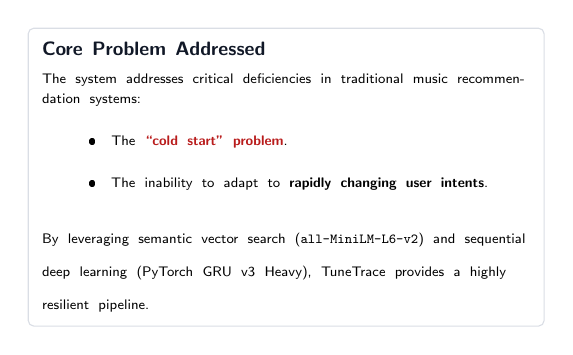
\begin{tikzpicture}
                \node[draw=inkRule, fill=white, rounded corners=2pt, text width=6.2cm, inner sep=5pt] {
                    {\fontsize{7pt}{8.5pt}\selectfont\bfseries\color{inkBlack}Core Problem Addressed}\\[3pt]
                    {\fontsize{5.5pt}{7.2pt}\selectfont
                    The system addresses critical deficiencies in traditional music recommendation systems:
                    \begin{itemize}
                        \item The \textbf{\color{focusRed}``cold start'' problem}.
                        \item The inability to adapt to \textbf{rapidly changing user intents}.
                    \end{itemize}
                    By leveraging semantic vector search (\texttt{all-MiniLM-L6-v2}) and sequential deep learning (PyTorch GRU v3 Heavy), TuneTrace provides a highly resilient pipeline.}
                };
            \end{tikzpicture}
            
            \vspace{0.15cm}
            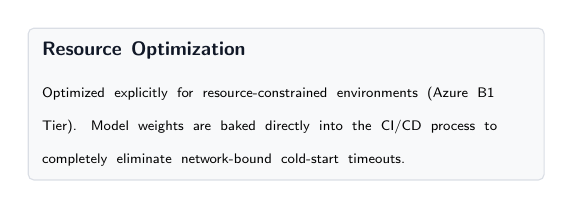
\begin{tikzpicture}
                \node[draw=inkRule, fill=inkLight, rounded corners=2pt, text width=6.2cm, inner sep=5pt] {
                    {\fontsize{7pt}{8.5pt}\selectfont\bfseries\color{inkBlack}Resource Optimization}\\[3pt]
                    {\fontsize{5.5pt}{7.2pt}\selectfont
                    Optimized explicitly for resource-constrained environments (Azure B1 Tier). Model weights are baked directly into the CI/CD process to completely eliminate network-bound cold-start timeouts.}
                };
            \end{tikzpicture}
        \end{column}

        \begin{column}{0.48\textwidth}
            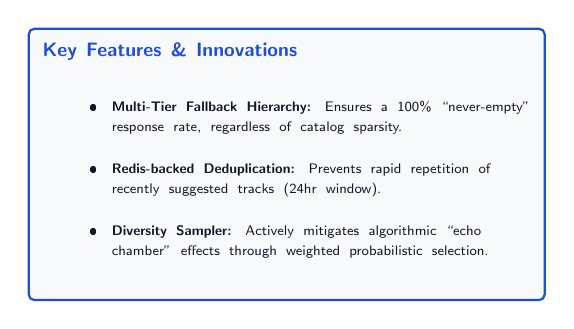
\begin{tikzpicture}
                \node[draw=focusBlue, fill=inkLight, rounded corners=2pt, line width=0.8pt, text width=6.2cm, inner sep=5pt] {
                    {\fontsize{7pt}{8.5pt}\selectfont\bfseries\color{focusBlue}Key Features \& Innovations}\\[3pt]
                    {\fontsize{5.5pt}{7.2pt}\selectfont\color{inkBlack}
                    \begin{itemize}
                        \item \textbf{Multi-Tier Fallback Hierarchy:} Ensures a 100\% ``never-empty'' response rate, regardless of catalog sparsity.
                        \item \textbf{Redis-backed Deduplication:} Prevents rapid repetition of recently suggested tracks (24hr window).
                        \item \textbf{Diversity Sampler:} Actively mitigates algorithmic ``echo chamber'' effects through weighted probabilistic selection.
                    \end{itemize}}
                };
            \end{tikzpicture}
        \end{column}
    \end{columns}
\end{frame}

% ==============================================================================
% SLIDE 3: SYSTEM OVERVIEW & CORE OBJECTIVES
% ==============================================================================
\section{1. System Overview}
\frametitle{Managing liked songs and generating suggestions via semantic \& sequential modeling}
\framesubtitle{Primary objectives and the underlying technical stack driving the TuneTrace ecosystem}

\begin{frame}
    \vspace{-0.1cm}
    \begin{columns}[T]
        \begin{column}{0.38\textwidth}
            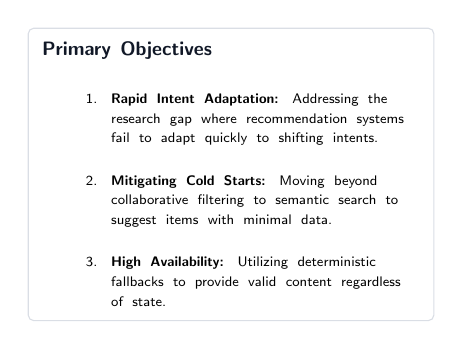
\begin{tikzpicture}
                \node[draw=inkRule, fill=white, rounded corners=2pt, text width=4.8cm, inner sep=5pt] {
                    {\fontsize{7pt}{8.5pt}\selectfont\bfseries\color{inkBlack}Primary Objectives}\\[3pt]
                    {\fontsize{5.5pt}{7.2pt}\selectfont
                    \begin{enumerate}
                        \item \textbf{Rapid Intent Adaptation:} Addressing the research gap where recommendation systems fail to adapt quickly to shifting intents.
                        \item \textbf{Mitigating Cold Starts:} Moving beyond collaborative filtering to semantic search to suggest items with minimal data.
                        \item \textbf{High Availability:} Utilizing deterministic fallbacks to provide valid content regardless of state.
                    \end{enumerate}}
                };
            \end{tikzpicture}
        \end{column}

        \begin{column}{0.58\textwidth}
            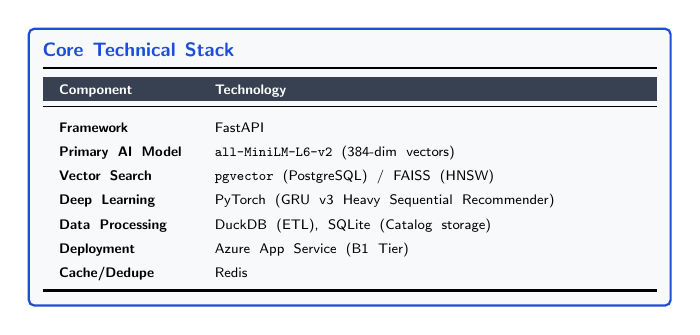
\begin{tikzpicture}
                \node[draw=focusBlue, fill=inkLight, rounded corners=2pt, line width=0.8pt, text width=7.8cm, inner sep=5pt] {
                    {\fontsize{7pt}{8.5pt}\selectfont\bfseries\color{focusBlue}Core Technical Stack}\\[3pt]
                    \fontsize{5.5pt}{7pt}\selectfont
                    \renewcommand{\arraystretch}{1.25}
                    \begin{tabularx}{\linewidth}{lX}
                        \toprule
                        \rowcolor{inkDark}
                        \textbf{\color{white}Component} & \textbf{\color{white}Technology} \\
                        \midrule
                        \textbf{Framework} & FastAPI \\
                        \textbf{Primary AI Model} & \texttt{all-MiniLM-L6-v2} (384-dim vectors) \\
                        \textbf{Vector Search} & \texttt{pgvector} (PostgreSQL) / FAISS (HNSW) \\
                        \textbf{Deep Learning} & PyTorch (GRU v3 Heavy Sequential Recommender) \\
                        \textbf{Data Processing} & DuckDB (ETL), SQLite (Catalog storage) \\
                        \textbf{Deployment} & Azure App Service (B1 Tier) \\
                        \textbf{Cache/Dedupe} & Redis \\
                        \bottomrule
                    \end{tabularx}
                };
            \end{tikzpicture}
        \end{column}
    \end{columns}
\end{frame}

% ==============================================================================
% SLIDE 4: RECOMMENDATION PIPELINE
% ==============================================================================
\section{2. Recommendation Pipeline}
\frametitle{A multi-tiered Version 3.0 pipeline engineered for deep semantic relevance and discovery}
\framesubtitle{Deconstructing the vectorization, user profiling, and active logic toggles}

\begin{frame}
    \vspace{-0.1cm}
    \begin{columns}[T]
        \begin{column}{0.48\textwidth}
            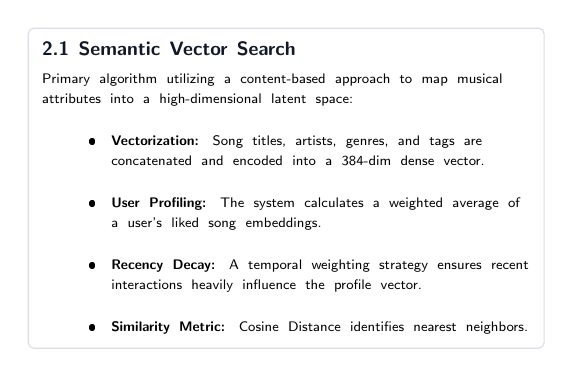
\begin{tikzpicture}
                \node[draw=inkRule, fill=white, rounded corners=2pt, text width=6.2cm, inner sep=5pt] {
                    {\fontsize{7pt}{8.5pt}\selectfont\bfseries\color{inkBlack}2.1 Semantic Vector Search}\\[3pt]
                    {\fontsize{5.5pt}{7.2pt}\selectfont
                    Primary algorithm utilizing a content-based approach to map musical attributes into a high-dimensional latent space:
                    \begin{itemize}
                        \item \textbf{Vectorization:} Song titles, artists, genres, and tags are concatenated and encoded into a 384-dim dense vector.
                        \item \textbf{User Profiling:} The system calculates a weighted average of a user’s liked song embeddings.
                        \item \textbf{Recency Decay:} A temporal weighting strategy ensures recent interactions heavily influence the profile vector.
                        \item \textbf{Similarity Metric:} Cosine Distance identifies nearest neighbors.
                    \end{itemize}}
                };
            \end{tikzpicture}
        \end{column}

        \begin{column}{0.48\textwidth}
            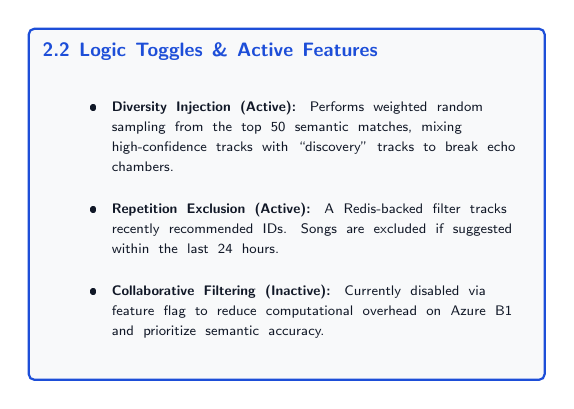
\begin{tikzpicture}
                \node[draw=focusBlue, fill=inkLight, rounded corners=2pt, line width=0.8pt, text width=6.2cm, inner sep=5pt] {
                    {\fontsize{7pt}{8.5pt}\selectfont\bfseries\color{focusBlue}2.2 Logic Toggles \& Active Features}\\[3pt]
                    {\fontsize{5.5pt}{7.2pt}\selectfont\color{inkBlack}
                    \begin{itemize}
                        \item \textbf{Diversity Injection (Active):} Performs weighted random sampling from the top 50 semantic matches, mixing high-confidence tracks with ``discovery'' tracks to break echo chambers.
                        \item \textbf{Repetition Exclusion (Active):} A Redis-backed filter tracks recently recommended IDs. Songs are excluded if suggested within the last 24 hours.
                        \item \textbf{Collaborative Filtering (Inactive):} Currently disabled via feature flag to reduce computational overhead on Azure B1 and prioritize semantic accuracy.
                    \end{itemize}}
                };
            \end{tikzpicture}
        \end{column}
    \end{columns}
\end{frame}

% ==============================================================================
% SLIDE 5: RESILIENCE & FALLBACK HIERARCHY
% ==============================================================================
\section{3. Resilience \& Fallback}
\frametitle{Ensuring 100\% availability through a deterministic four-tier fallback routing chain}
\framesubtitle{A structured "never-empty" response mechanism prioritizing semantic vectors down to global trends}

\begin{frame}
    \vspace{-0.1cm}
    \centering
    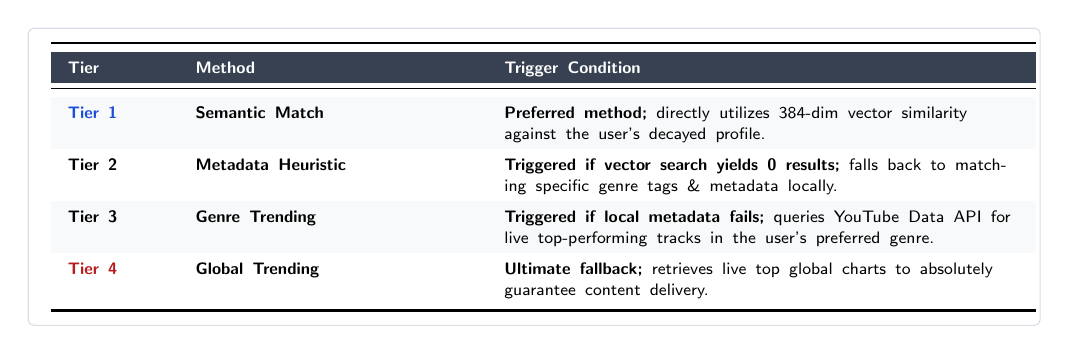
\begin{tikzpicture}
        \node[draw=inkRule, fill=white, rounded corners=2pt, text width=12.5cm, inner sep=5pt] {
            \fontsize{6pt}{7.5pt}\selectfont
            \renewcommand{\arraystretch}{1.5}
            \begin{tabularx}{\linewidth}{p{1.2cm}p{3.5cm}X}
                \toprule
                \rowcolor{inkDark}
                \textbf{\color{white}Tier} & \textbf{\color{white}Method} & \textbf{\color{white}Trigger Condition} \\
                \midrule
                \rowcolor{inkLight}
                \textbf{\color{focusBlue}Tier 1} & \textbf{Semantic Match} & \textbf{Preferred method;} directly utilizes 384-dim vector similarity against the user's decayed profile. \\
                \rowcolor{white}
                \textbf{Tier 2} & \textbf{Metadata Heuristic} & \textbf{Triggered if vector search yields 0 results;} falls back to matching specific genre tags \& metadata locally. \\
                \rowcolor{inkLight}
                \textbf{Tier 3} & \textbf{Genre Trending} & \textbf{Triggered if local metadata fails;} queries YouTube Data API for live top-performing tracks in the user's preferred genre. \\
                \rowcolor{white}
                \textbf{\color{focusRed}Tier 4} & \textbf{Global Trending} & \textbf{Ultimate fallback;} retrieves live top global charts to absolutely guarantee content delivery. \\
                \bottomrule
            \end{tabularx}
        };
    \end{tikzpicture}
\end{frame}

% ==============================================================================
% SLIDE 6: INTENT STATE MODELING & SEQUENTIAL RECOMMENDER
% ==============================================================================
\section{4. Intent State Modeling}
\frametitle{The Samsung PRISM Sandbox isolates sequential user tracking across the YAMDA-50M dataset}
\framesubtitle{Scaling ETL pipelines, comparing heuristic engines with the upgraded v3 Heavy PyTorch model}

\begin{frame}
    \vspace{-0.1cm}
    \begin{columns}[T]
        \begin{column}{0.48\textwidth}
            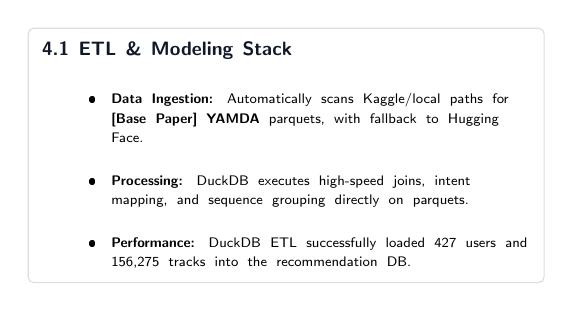
\begin{tikzpicture}
                \node[draw=inkRule, fill=white, rounded corners=2pt, text width=6.2cm, inner sep=5pt] {
                    {\fontsize{7pt}{8.5pt}\selectfont\bfseries\color{inkBlack}4.1 ETL \& Modeling Stack}\\[3pt]
                    {\fontsize{5.5pt}{7.2pt}\selectfont
                    \begin{itemize}
                        \item \textbf{Data Ingestion:} Automatically scans Kaggle/local paths for \textbf{[Base Paper] YAMDA} parquets, with fallback to Hugging Face.
                        \item \textbf{Processing:} DuckDB executes high-speed joins, intent mapping, and sequence grouping directly on parquets.
                        \item \textbf{Performance:} DuckDB ETL successfully loaded 427 users and 156,275 tracks into the recommendation DB.
                    \end{itemize}}
                };
            \end{tikzpicture}
            
            \vspace{0.15cm}
            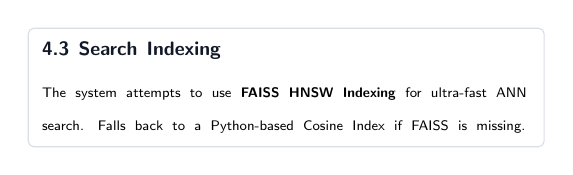
\begin{tikzpicture}
                \node[draw=inkRule, fill=white, rounded corners=2pt, text width=6.2cm, inner sep=5pt] {
                    {\fontsize{7pt}{8.5pt}\selectfont\bfseries\color{inkBlack}4.3 Search Indexing}\\[3pt]
                    {\fontsize{5.5pt}{7.2pt}\selectfont
                    The system attempts to use \textbf{FAISS HNSW Indexing} for ultra-fast ANN search. Falls back to a Python-based Cosine Index if FAISS is missing.}
                };
            \end{tikzpicture}
        \end{column}

        \begin{column}{0.48\textwidth}
            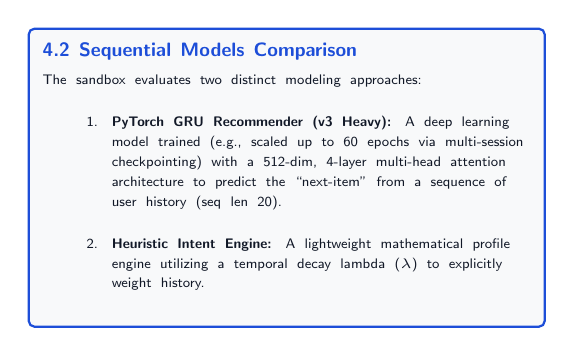
\begin{tikzpicture}
                \node[draw=focusBlue, fill=inkLight, rounded corners=2pt, line width=0.8pt, text width=6.2cm, inner sep=5pt] {
                    {\fontsize{7pt}{8.5pt}\selectfont\bfseries\color{focusBlue}4.2 Sequential Models Comparison}\\[3pt]
                    {\fontsize{5.5pt}{7.2pt}\selectfont\color{inkBlack}
                    The sandbox evaluates two distinct modeling approaches:
                    \begin{enumerate}
                        \item \textbf{PyTorch GRU Recommender (v3 Heavy):} A deep learning model trained (e.g., scaled up to 60 epochs via multi-session checkpointing) with a 512-dim, 4-layer multi-head attention architecture to predict the ``next-item'' from a sequence of user history (seq len 20).
                        \item \textbf{Heuristic Intent Engine:} A lightweight mathematical profile engine utilizing a temporal decay lambda ($\lambda$) to explicitly weight history.
                    \end{enumerate}}
                };
            \end{tikzpicture}
        \end{column}
    \end{columns}
\end{frame}

% ==============================================================================
% SLIDE 7: API ARCHITECTURE & DEPLOYMENT
% ==============================================================================
\section{5. API Architecture}
\frametitle{A lightweight, high-performance FastAPI microservice constrained for Azure B1 Tier hardware}
\framesubtitle{Endpoint contracts, data schema, and optimizations mitigating network-bound delays}

\begin{frame}
    \vspace{-0.1cm}
    \begin{columns}[T]
        \begin{column}{0.48\textwidth}
            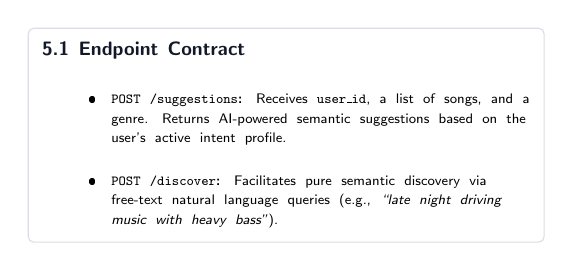
\begin{tikzpicture}
                \node[draw=inkRule, fill=white, rounded corners=2pt, text width=6.2cm, inner sep=5pt] {
                    {\fontsize{7pt}{8.5pt}\selectfont\bfseries\color{inkBlack}5.1 Endpoint Contract}\\[3pt]
                    {\fontsize{5.5pt}{7.2pt}\selectfont
                    \begin{itemize}
                        \item \textbf{\texttt{POST /suggestions}:} Receives \texttt{user\_id}, a list of songs, and a genre. Returns AI-powered semantic suggestions based on the user's active intent profile.
                        \item \textbf{\texttt{POST /discover}:} Facilitates pure semantic discovery via free-text natural language queries (e.g., \textit{``late night driving music with heavy bass''}).
                    \end{itemize}}
                };
            \end{tikzpicture}
            
            \vspace{0.15cm}
            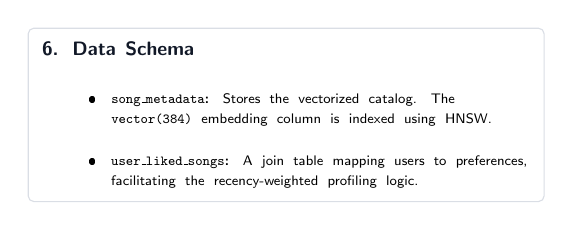
\begin{tikzpicture}
                \node[draw=inkRule, fill=white, rounded corners=2pt, text width=6.2cm, inner sep=5pt] {
                    {\fontsize{7pt}{8.5pt}\selectfont\bfseries\color{inkBlack}6. Data Schema}\\[3pt]
                    {\fontsize{5.5pt}{7.2pt}\selectfont
                    \begin{itemize}
                        \item \textbf{\texttt{song\_metadata}:} Stores the vectorized catalog. The \texttt{vector(384)} embedding column is indexed using HNSW.
                        \item \textbf{\texttt{user\_liked\_songs}:} A join table mapping users to preferences, facilitating the recency-weighted profiling logic.
                    \end{itemize}}
                };
            \end{tikzpicture}
        \end{column}

        \begin{column}{0.48\textwidth}
            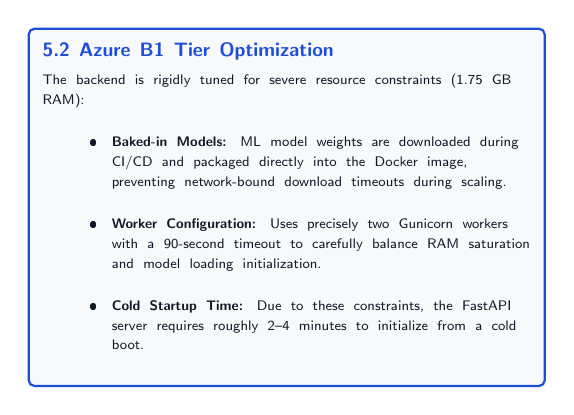
\begin{tikzpicture}
                \node[draw=focusBlue, fill=inkLight, rounded corners=2pt, line width=0.8pt, text width=6.2cm, inner sep=5pt] {
                    {\fontsize{7pt}{8.5pt}\selectfont\bfseries\color{focusBlue}5.2 Azure B1 Tier Optimization}\\[3pt]
                    {\fontsize{5.5pt}{7.2pt}\selectfont\color{inkBlack}
                    The backend is rigidly tuned for severe resource constraints (1.75 GB RAM):
                    \begin{itemize}
                        \item \textbf{Baked-in Models:} ML model weights are downloaded during CI/CD and packaged directly into the Docker image, preventing network-bound download timeouts during scaling.
                        \item \textbf{Worker Configuration:} Uses precisely two Gunicorn workers with a 90-second timeout to carefully balance RAM saturation and model loading initialization.
                        \item \textbf{Cold Startup Time:} Due to these constraints, the FastAPI server requires roughly 2--4 minutes to initialize from a cold boot.
                    \end{itemize}}
                };
            \end{tikzpicture}
        \end{column}
    \end{columns}
\end{frame}

\end{document}
